% Chapter Template

\chapter{Research proposal}\label{chapter:firstchapter} % Main chapter title

\label{ChapterX} % Change X to a consecutive number; for referencing this chapter elsewhere, use \ref{ChapterX}

%----------------------------------------------------------------------------------------
%	SECTION 1
%----------------------------------------------------------------------------------------

\section{Introduction}\label{sec:firstsection}


% It is a good idea to have each sentence on a separate line, so that if you get feedback or changes from someone else
% the diffs will be much easier to manage
In this technological driven era, due to new technical advancements been made in collaboration with human ability, many products are available that uses technology for satisfying the need of people, still there exists a gap between technology and areas where people are completely isolated to communicate with rest part of the world, interaction to get aware of what is going around in the world, is thus prime importance for vulnerable population. However, the trends are certainly going to change as we are coming up with an innovative and economically feasible concept of providing tsunami alert using a system of an advanced technology, so called ETC-Lali Low-Cost Communications and All-Hazard Early Warning System, it is thus claimed that this system can be the future of indo-pacific region.

\begin{figure}
\begin{centering}


\label{fig:ThisFig}
\end{centering}
\end{figure}

%-----------------------------------
%	SUBSECTION 1
%-----------------------------------
\subsection{Problem/Research Question/Project Focus  }
the problem arises as people living in coastal areas do not have economical viable system for tsunami which can be  bought as it costs a handsome amount of money to purchase install and maintain the system. So our project is aiming to provide the solution which can be economical for people to purchase and install it.The main focus of the project is to provide direct link and providing them awareness of whats going around the world including tsunami alerts to vulnerable population living in isolated islands and other area which are completely excluded from the rest part of world.\\

The project aims to provide awareness to that part of area and will keep the locals update in their locality as ETC-Lali system will not only provide the alerts for tsunami, but at the same time providing the full entertainment by playing music and keeping them update by streaming daily news through radio programming.


%-----------------------------------
%	SUBSECTION 2
%-----------------------------------

\subsection{ Background surveys}
The first survey was regarded the occurrence of natural disasters Natural disasters that posed largest threat to the life of people living on earth in the past. Certainly, the region that records highest number of natural disasters on earth\\
 According to study of mental health ASIA, Indo pacific region specifically Asia is among the highest natural disaster prone area on planet earth, there are assorted reasons, out of them is the geographical location as eastern and south east countries lies   on pacific seismic belt  from Aleutian trench to Mariana trench, Likewise Eurasian plate is situated on Indian platesSo whenever a collision occurs in between these plates, there has been high destruction earthquakes causing damaging to human life and causing tsunami. \\

Another, study of reference ind author endnote revealed the real world example of destruction caused by tsunami waves in Japan which killed above 15,000 people and costing the country economically around 235 billion dollars. Although there exists many multi-hazard warning systems but the working, cost and maintenance of those systems can be covered by large organisation or government firms as large amount of money is required.\\

The third paper according to ind author  illustrates a clear example of warning system in India, Tsunami warning system was installed in the year 2011 wnhich is known as (IOTWMS) Indian Ocean Tsunami Warning and Mitigation System where twenty four centres for warnings in Indian oceans were setup. The systems are working, However the risk of coastal hazards still cannot be successfully minimised as there were barriers in communication of warning which does not even reached to vulnerable population, other reasons were data collection and gathering of messages and lastly the lack of devices and equipment’s in the region.  
%----------------------------------------------------------------------------------------
%	SECTION 2
%----------------------------------------------------------------------------------------

\section{Group member roles}

This is the joint statement of our group member "The ETC Lali system consists of three main parts, A receiver that contains a siren and FM radio transmitter portal that provides useful radio programming during peace time, a disaster management portal that allows the definition and dispatch of tsunami and other warnings, and a portal that allows for the injection and management of the radio audio streams."\\

This project concerns that third part. The goal of the project is to identify and document the requirements of the radio audio injection portal, so that it provides all of the required functionality for a commercial radio station to easily contribute content to the ETC Lali system\\
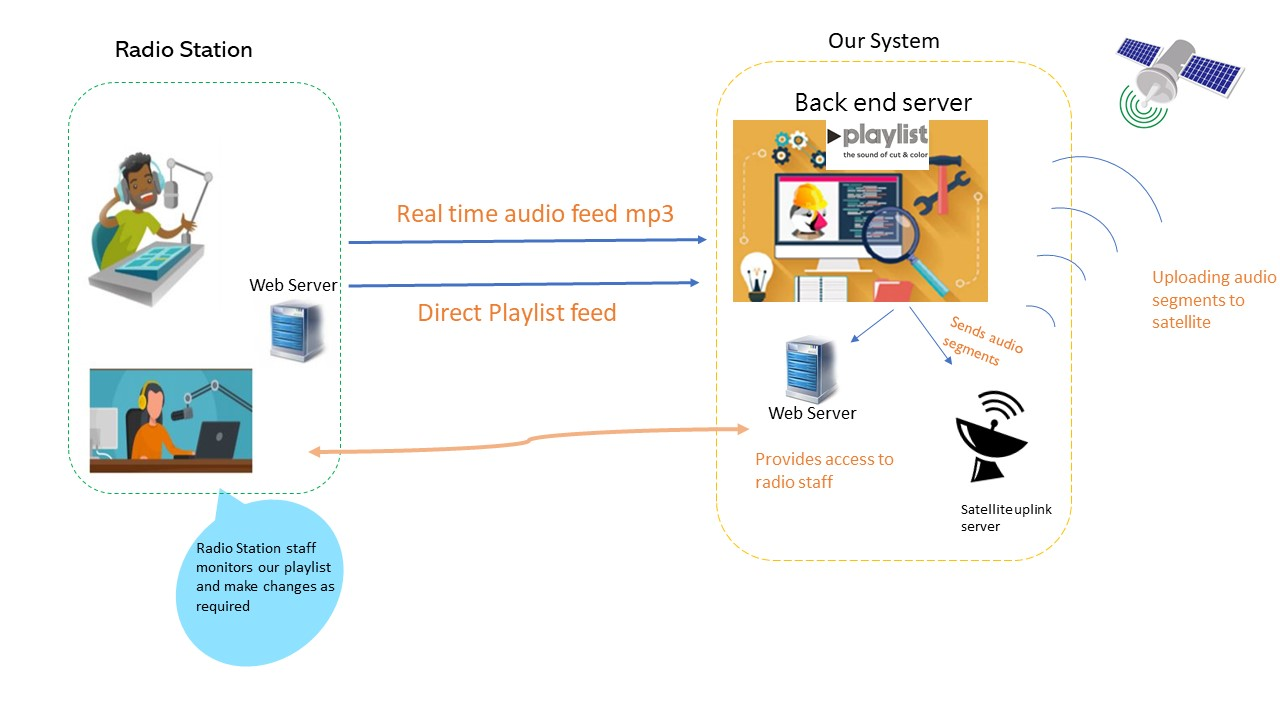
\includegraphics[width=15cm,height=15cm,keepaspectratio]{Figures/1.jpg}\\
\caption{Figure A: hows the working of radio transmitter injection portal}

In this project my role is to provide direct engagement with commercial radio station. I will be developing a user interface audio injection web portal which will be having a back-end server delivering the radio streams received directly from radio station team and providing management services and injection operation required during disaster thus delivering the stream signal to satellite through a server which will be sending streams to receiver side via satellite where the end product is installed in a particular island.\\

We have been in contact with one of radio station team in Adelaide who are ready to share their audio cards and audio management data processing strategies required for progression of our project.The clear in-depth working of my role will be taking the audio stream from commercial radio station.The audio stream received can follow two assorted approaches namely real time audio or a full playlist of audio stream. The real time audio involves the live stream music channel which is broadcasted live on radio station.\\

The second method which is preferred the most is requesting the entire playlist from radio station department.The playlist will be having a list of music that will be playing regularly divided into morning, afternoon, evening, and night intervals respectively including the news updates.The worse case scenario is if for any reason, playlist is not available, then a music recognition programming and algorithms concepts can be developed to automatically recognise the currently playing music live on radio station on the internet.\\
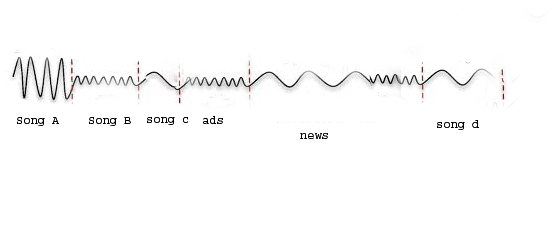
\includegraphics[width=15cm,height=15cm,keepaspectratio]{Figures/3.jpg}\\ Figure b) illustrates the radio stream management and operations for the playlist\\

Once a radio station team provided us the playlist , my role will be to manage the  live stream of playlist as downloading the file would be resulting in time delay, so we will use online stream playlist which does not require downloading , instead can be played online, managing the  playlist is of immense importance as various operations like sending the received tracks in piece of segments  will be our motive.\\
 In figure b) it is apparent  by assuming that songs a,b,c along with ads will be sent to server  which will upload that segments till then news will be broadcasted  again another segment will be uploaded to satellite with the following songs in the playlist .The audio tracks will be uploaded in different pieces as the satellite can only upload up to 200 bytes per second. But the audio stream is of 2 kilo bytes per second  so we can send only audio which is one tenth of the time  to upload to the satellite due to this reason the audio needs to be sent in segments.\\
 In addition, we can only stream every hour of audio up to 10 minutes real time audio, in the mean time rest of  playlist,s information will be streamed. Our system can inject self recorded audio messages along with the playlist. For instance, disaster management department receives the update on tsunami coming towards a certain region. In that case, our system will be able to send pre-recorded messages to the server via satellite which will inform receiver part, therefore alarming the sirens and providing the warning to locals to that designated location.

